\documentclass[11pt, oneside]{article}   	% use "amsart" instead of "article" for AMSLaTeX format
\usepackage{geometry}                		% See geometry.pdf to learn the layout options. There are lots.
\geometry{letterpaper}                   		% ... or a4paper or a5paper or ... 
%\geometry{landscape}                		% Activate for for rotated page geometry
%\usepackage[parfill]{parskip}    		% Activate to begin paragraphs with an empty line rather than an indent
\usepackage{graphicx}				% Use pdf, png, jpg, or eps� with pdflatex; use eps in DVI mode
								% TeX will automatically convert eps --> pdf in pdflatex		
\usepackage{amssymb}
\usepackage{amsmath}
\usepackage{parskip}
\usepackage{color}

\title{Examples for Green's theorem (work)}
%\author{The Author}
%\section{}
% \subsection*{R code}
\date{}							% Activate to display a given date or no date

\graphicspath{{/Users/telliott_admin/Dropbox/Tex/png/}}

% \begin{center} 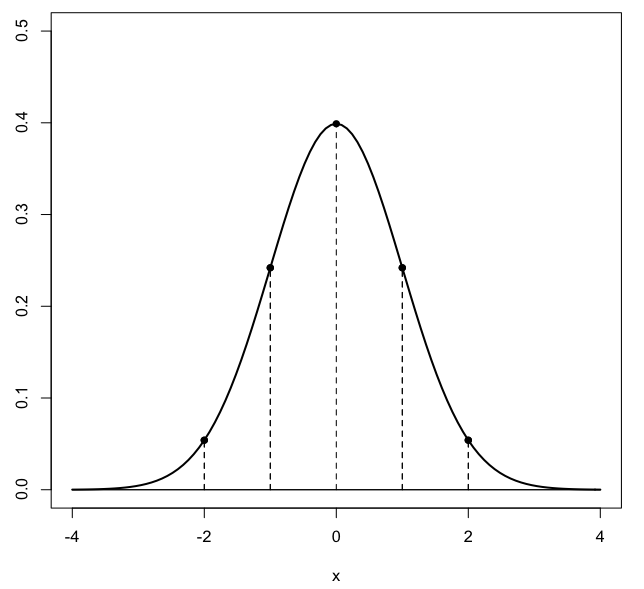
\includegraphics [scale=0.4] {gauss3.png} \end{center}
% \begin{bmatrix} a  &  b \\ c  &  d \end{bmatrix}
% \bigg |_

\begin{document}
\maketitle
\large
%\noindent
State the theorem:
\[ \oint_C \mathbf{F} \cdot \mathbf{r} = \iint_R \nabla \times \mathbf{F} \ dA \]
\[ \int_C M \ dx + N \ dy = \iint_R (N_x - M_y) \ dx \ dy \]

To start with, if $\mathbf{F}$ is the gradient of some function, we call such a function the potential, and the integral of the work over a closed path is just zero.

\[ \mathbf{F} = \ <y,x> \]
\[ f = xy \]
Suppose we take the line integral of $\mathbf{F}\cdot \mathbf{r}$  over the unit square $(0,0)$ to $(0,1)$, etc.
\[ \oint_C y \ dx + x \ dy = \]
I get $0 + 1 -1 + 0 = 0$.

A sign change can make all the difference.
\[ \mathbf{F} = \ <-y,x> \]
\[ N_x - M_y = 1 - -1 = 2 \ne 0 \]

A common field with zero curl in 3D is
\[ \mathbf{F} = \ <yz,xz,xy> \]
\[ \nabla \times \mathbf{F} = \ <R_y-Q_z,P_z-R_x,Q_x-P_y> \]
\[ = x - x, y - y, z - z > \ = \mathbf{0} \]

\subsection*{Auroux}
Suppose 
\[ \mathbf{F} = \ <ye^{-x},\frac{1}{2}x^2 - e^{-x}> \]
And suppose further that the region is the unit disk centered at $(2,0)$  The line integral does not look like fun, and the region is no help, but 
\[ N_x - M_y = x + e^{-x} - e^{-x} = x \]
So the integral of the curl is just
\[ \iint_R x \ dA \]
which is $\overline{x}$ on this disk, which is just equal to $2$ by symmetry.

\subsection*{Paul}
Given 
\[ \mathbf{F} = \ <xy,x^2y^3> \]
The curl is
\[ N_x - M_y = 2xy^3 - x \]
If the region is the triangle $(0,0) \rightarrow (1,0) \rightarrow (1,2) \rightarrow (0,0)$ then
\[ \int_0^1 \int_0^{2x} 2xy^3 - x \ dy \ dx \]
inner
\[ = \frac{1}{2}xy^4 - xy \ \bigg |_0^{2x} = 8x^5 - 2x^2 \]
outer
\[ \int_0^1 8x^5 - 2x^2 \ dx = \frac{8}{6}x^6 - \frac{2}{3}x^3 \bigg |_0^1 = \frac{8}{6} - \frac{2}{3} = \frac{2}{3} \]
Try the line integral to check it.

\subsection*{ellipse}
Of course, my favorite example is the area of the ellipse.  Suppose $N_x - M_y = 1$.  Then the curl integral is the area of the region.  If the components of $\mathbf{F}$ are $N = x/2$ and $M=-y/2$, this condition holds.  Parametrize the ellipse.
\[ x = a \cos \theta \]
\[ y = b \sin \theta \]
So, for the left hand side we have
\[ \int_C M \ dx + N \ dy = \int_C -\frac{1}{2}y \ dx + \frac{1}{2}x \ dy \]
\[ = \int_0^{2\pi} (-\frac{1}{2})(b \sin \theta) \ (-a \sin \theta) \ d \theta \ + (\frac{1}{2})(a \cos \theta) \ (b \cos \theta) \ d\theta \]
\[ = \frac{1}{2} ab \int_0^{2\pi} \sin^2 \theta \ d \theta +  \int_0^{2\pi} \cos^2 \theta \ d \theta \]
\[ = \frac{1}{2} ab \int_0^{2\pi} \ d \theta = \pi a b\]

You may wonder why we chose $\mathbf{F} = \ \langle -y/2, x/2 \rangle$ since there are many other values that would work.  The reason is that the integral is particularly easy.  Let's try one other choice:
\[ \mathbf{F} = \ \langle 0, x \rangle \]
We use the same parametrization from above.  The left hand side is:
\[ \int_C M \ dx + N \ dy = \int_C 0 \ dx + x \ dy \]
\[ =  \int_0^{2\pi} a \cos \theta \ b \cos \theta \ d \theta \]
\[ = ab \int_0^{2\pi}  \cos^2 \theta \ d \theta \]
\[ = \frac{1}{2} a b \ (\theta + \sin \theta \cos \theta) | \bigg |_0^{2\pi}  ) \]
\[ = \pi a b \]


\end{document}  